\documentclass{beamer}
%\usepackage{longtable}
%\usepackage{graphicx}
%\usepackage{afterpage}
\usepackage[T1]{fontenc}
\usepackage[utf8]{inputenc}
\usepackage{appendixnumberbeamer}

\usepackage{booktabs}
\usepackage{tabularx}
\usepackage{listings}
\usepackage{amsmath}
\usepackage{graphicx}
\usepackage{algorithmic}
\usepackage{algorithm2e}
\usepackage{cancel}
\usepackage{listings}
\usepackage{caption}


%\usefonttheme{structuresmallcapsserif}
\usefonttheme{structurebold}
\usetheme{Marburg}
%\usecolortheme{crane}
%\usetheme{Malmoe}
%\usetheme{Dresden} 


\makeatletter
  \setbeamertemplate{sidebar \beamer@sidebarside}
  {
    \beamer@tempdim=\beamer@sidebarwidth%
    \advance\beamer@tempdim by -6pt%
    \vskip4em%
    \insertverticalnavigation{\beamer@sidebarwidth}%
    \vfill
    \ifx\beamer@sidebarside\beamer@lefttext%
    \else%
      \usebeamercolor{normal text}%
      \llap{\usebeamertemplate***{navigation symbols}\hskip0.1cm}%
      \vskip2pt%
    \fi%
  }%

  \ifx\beamer@sidebarside\beamer@lefttext%
    \defbeamertemplate*{sidebar right}{sidebar theme}
    {%
      \vfill%
      \llap{\usebeamertemplate***{navigation symbols}\hskip0.1cm}%
      \vskip2pt}
  \fi

\setbeamertemplate{section in sidebar}%{sidebar theme}
{%
  \vbox{%
    \vskip1ex%
    \beamer@sidebarformat{3pt}{section in sidebar}{\insertsectionheadnumber
~\insertsectionhead}%
  }%
}
\setbeamertemplate{section in sidebar shaded}%{sidebar theme}
{%
  \vbox{%
    \vskip1ex%
    \beamer@sidebarformat{3pt}{section in sidebar shaded}{\insertsectionheadnumber
~\insertsectionhead}%
  }%
}
\makeatother
 
%gets rid of bottom navigation symbols
\setbeamertemplate{navigation symbols}{}

%gets rid of footer
%will override 'frame number' instruction above
%comment out to revert to previous/default definitions
\setbeamertemplate{footline}{} 
 
%Information to be included in the title page:
\title{Inverzna kinematika manipulatora ostvarena pomoću dubokog potpornog učenja }
\author{Autor: Josip Torić \\ Mentor: izv. prof. dr. sc.~Marija Seder}
\date{10. srpnja 2020.}
\institute{Fakultet elektrotehnike i računarstva, Sveučilište u Zagrebu}
 
%\logo{\includegraphics[height=1.5cm]{lion-logo.png}}

\AtBeginSection[]
{
  \begin{frame}
    \frametitle{Sadržaj}
    \tableofcontents[currentsection,currentsubsection]
  \end{frame}
}
 
\begin{document}

\frame{\titlepage}

\begin{frame}
	\frametitle{Sadržaj}
	\tableofcontents
\end{frame}

\section{Uvod}

\begin{frame}
	\frametitle{Uvod}

	Živimo u svijetu prepunom informacija, zadataka i problema.
	\bigskip

	Znanstvenici su nakon Drugog svjetskog rata krenuli razvijati umjetnu inteligenciju iz koje su se kasnije razvili strojno učenje, duboko učenje i potporno učenje.
	\bigskip

	Cilj ovog diplomskog rada je naučiti inverznu kinematiku robotske ruke Jaco uz primjenu dubokog potpornog učenja.

\end{frame}

\section{Teorijske osnove potpornog učenja}
\subsection{Potporno učenje}

\begin{frame}
	\frametitle{Koncept potpornog učenja}

	Potporno učenje je grana strojnog učenja koja proučava agente i kako oni uče na temelju pokušaja i pogreške.
	\bigskip

	Osnovna ideja potpornog učenja je da postoji agent u svojem okruženju.

\end{frame}


\begin{frame}
	\frametitle{Odnos agenta i okruženja}

	\begin{figure}[h!]
		\centering
		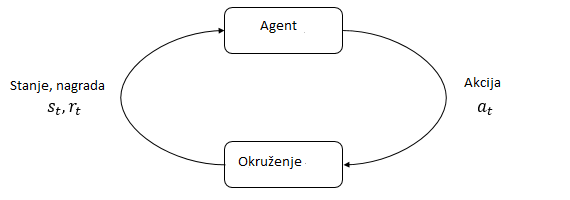
\includegraphics[width=\columnwidth]{img/agent-environment.png}
		\label{fig:agenta}
	\end{figure}
	\footnotetext{Preuzeto sa \url{https://spinningup.openai.com}}


\end{frame}


\begin{frame}
	\frametitle{Duboko potporno učenje}
	Politike odabira akcija u potpornom učenju se spremaju u funkcije.
	\bigskip

	No, kao i svaka funkcija ona je ograničena s parametrima i klasom funkcija koje pripada. Zbog toga u prošlosti, potporno učenje je imalo limitirane primjene.
	\bigskip

	Pravi proboj u potpornom učenju se dogodio kada su počeli umjesto funkcija aproksimirati dubokim neuronskim mrežama.

\end{frame}


\subsection{Teoretska pozadina potpornog učenja}

\begin{frame}
	\frametitle{Osnovni pojmovi potpornog učenja}

	\begin{itemize}
		\item Prostor opservacija
		\item Prostor akcija
		\item Politika
		\item Putanja
		\item Nagrada
	\end{itemize}

\end{frame}

\begin{frame}
	\frametitle{Problem potpornog učenja}

	Problem potpornog učenja je odabrati optimalnu politiku koja će maksimizirati očekivanu nagradu.
	\bigskip

	\begin{equation}
		\label{probability trajectory}
		P(\tau|\pi) = \rho_0 (s_0) \prod_{t=0}^{T-1} P(s_{t+1} | s_t, a_t) \pi(a_t | s_t)
	\end{equation}

	\begin{equation}
		\label{ukupna nagrada}
		J(\pi) = \int_{\tau} P(\tau|\pi) R(\tau) = \underset{\tau\sim \pi} E[{R(\tau)}]
	\end{equation}

	\begin{equation}
		\label{optimizacijski problem}
		\pi^* = \arg \max_{\pi} J(\pi)
	\end{equation}

\end{frame}



\begin{frame}
	\frametitle{Vrijednosne funkcije}

	\begin{equation}
		\label{prva vrijednosna}
		V^{\pi}(s) = \underset{\tau \sim \pi}E[{R(\tau)\left| s_0 = s\right.}]
	\end{equation}

	\begin{equation}
		\label{druga vrijednosna}
		Q^{\pi}(s,a) = \underset{\tau \sim \pi}E[{R(\tau)\left| s_0 = s, a_0 = a\right.}]
	\end{equation}

	\begin{equation}
		\label{treća vrijednosna}
		V^*(s) = \max_{\pi} \underset{\tau \sim \pi}E[{R(\tau)\left| s_0 = s\right.}]
	\end{equation}

	\begin{equation}
		\label{četvrta vrijednosna}
		Q^*(s,a) = \max_{\pi} \underset{\tau \sim \pi}E[{R(\tau)\left| s_0 = s, a_0 = a\right.}]
	\end{equation}

	\begin{equation}
		A^{\pi}(s,a) = Q^{\pi}(s,a) - V^{\pi}(s)
	\end{equation}

\end{frame}

\begin{frame}
	\frametitle{Bellmanove jednadžbe}

	\begin{equation}
		\label{belman 1}
		V^{\pi}(s) = \underset{s'\sim P}E[{r(s,a) + \gamma V^{\pi}(s')}]
	\end{equation}

	\begin{equation}
		\label{belman 2}
		Q^{\pi}(s,a) = \underset{s'\sim P}E[{r(s,a) + \gamma \underset{a'\sim \pi}E[{Q^{\pi}(s',a')}}]]
	\end{equation}

	\begin{equation}
		\label{belman 3}
		V^*(s) = \max_a \underset{s'\sim P}E[{r(s,a) + \gamma V^*(s')}]
	\end{equation}

	\begin{equation}
		\label{belman 4}
		Q^*(s,a) = \underset{s'\sim P}E[{r(s,a) + \gamma \max_{a'} Q^*(s',a')}]
	\end{equation}

\end{frame}

\subsection{Podjela algoritama potpornog učenja}

\begin{frame}
	\frametitle{Podjela algoritama potpornog učenja}

	\begin{figure}[h!]
		\centering
		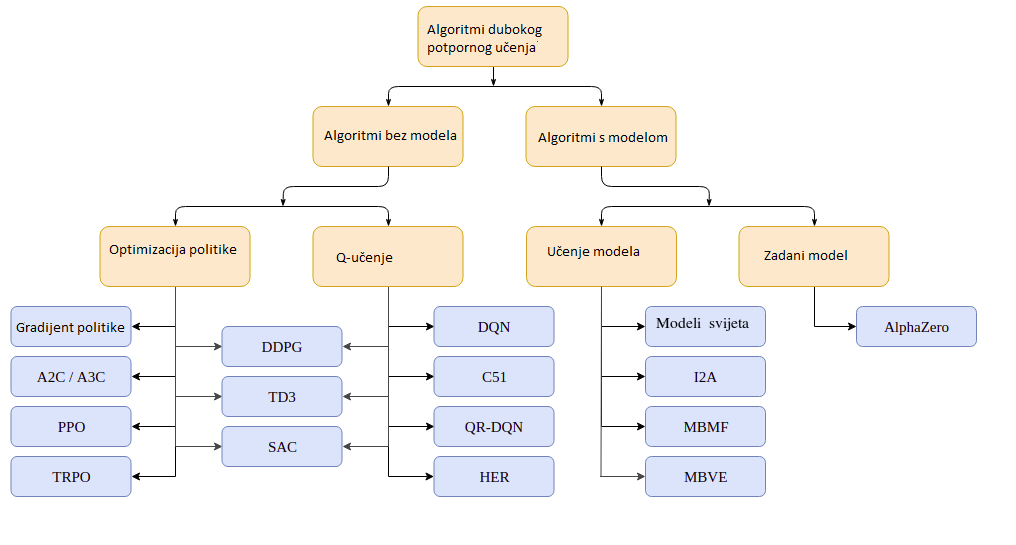
\includegraphics[width=\columnwidth]{img/podjela.png}
		\label{fig:podjela}
	\end{figure}
	\footnotetext{Preuzeto sa \url{https://spinningup.openai.com}}

\end{frame}

\section{Praktične primjene potpornog učenja}

\begin{frame}
	\frametitle{Primjene u igranju šaha}

	Postoji otprilike ${10^{120}}$ mogućih šahovskih partija.
	\bigskip

	Većina današnjih računalnih programa za igranje šaha počiva na nekom principu pretraživanja prostora.
	\bigskip

	Algoritmi bazirani na dubokom potpornom učenju, kao što su AlphaZero i Leela Chess Zero, uspjeli su kombinirati računalnu snagu s ljudskom intuicijom.

\end{frame}

\begin{frame}
	\frametitle{Primjene u igranju računalnih igara}

	Računalne igre, za razliku od igara na ploči, su korak bliže realnom svijetu.
	\bigskip

	Vjerojatno jedna od najpoznatijih primjena dubokog potpornog učenja u zadnje vrijeme je kada je skupina znanstvenika okupljena u OpenAI timu razvila botove koji su postali bolji od svjetskih prvaka u računalnoj igri Dota 2.
	\bigskip

	Također, jedan od čestih benchmarkova za evaluiranje rada algoritama je igranje igara na konzoli Atari 2600.

\end{frame}

\begin{frame}
	\frametitle{Atari 2600}

	\begin{figure}[ht!]
		\centering
		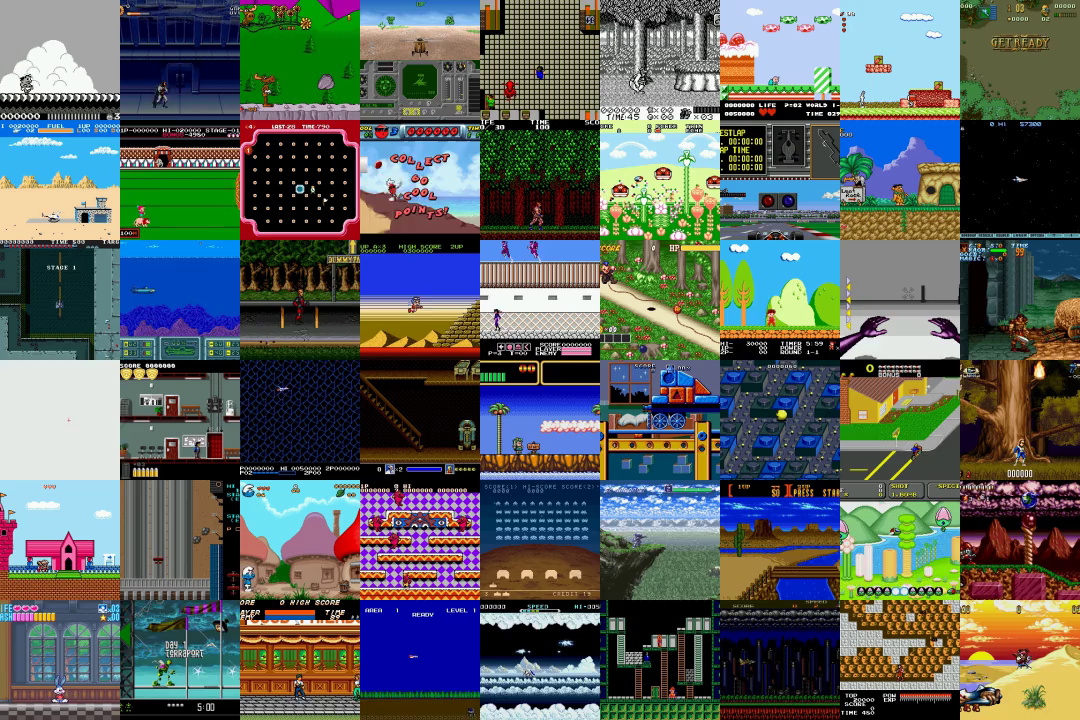
\includegraphics[width=\columnwidth]{img/atari.png}
		\label{fig:atari}
	\end{figure}
	\footnotetext{Preuzeto sa \url{https://openai.com}}
\end{frame}

\begin{frame}
	\frametitle{Primjene u robotici}

	Kod robota okruženje je stvarni svijet i njihove akcije imaju posljedice u stvarnom svijetu.
	\bigskip

	Robotu su najčešće dostupne informacije o položaju u kojem se nalazi, zatim o kutevima zglobova koji ga pokreću, trenutnoj brzini, itd.
	\bigskip

	Jedan od najvećih problema vezano za robotiku je nepraktičnost treniranja robota.
	\bigskip

	Glavni zadatak ovog diplomskog rada je naučiti inverznu kinematiku robotske ruke Jaco prilikom dohvaćanja loptice iz okruženja, prvo bez prepreka te zatim s preprekama

\end{frame}

\section{Algoritmi optimizacije politike}

\begin{frame}
	\frametitle{Pregled algoritama optimizacije politike}

	Najosnovniji algoritam optimizacije politike je algoritam jednostavnog gradijenta politike, ali problem kod njega je prevelika nestabilnost.
	\bigskip

	Zbog toga ću iznijeti još dva algoritma, algoritam optimizacije politike uz regije povjerenja i algoritam proksimalne optimizacije politike.
\end{frame}

\subsection{Algoritam jednostavnog gradijenta politike}

\begin{frame}
	\frametitle{Algoritam jednostavnog gradijenta politike}

	\begin{figure}[h!]
		\centering
		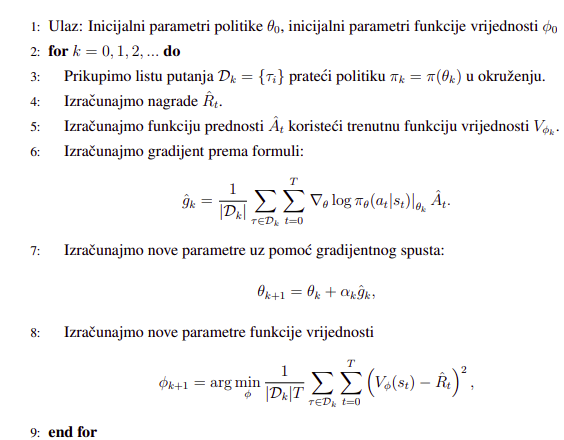
\includegraphics[width=\columnwidth]{img/vpg.png}
	\end{figure}

\end{frame}


\subsection{Algoritam optimizacije politike uz regije povjerenja}

\begin{frame}
	\frametitle{Algoritam optimizacije politike uz regije povjerenja}

	\begin{figure}[h!]
		\centering
		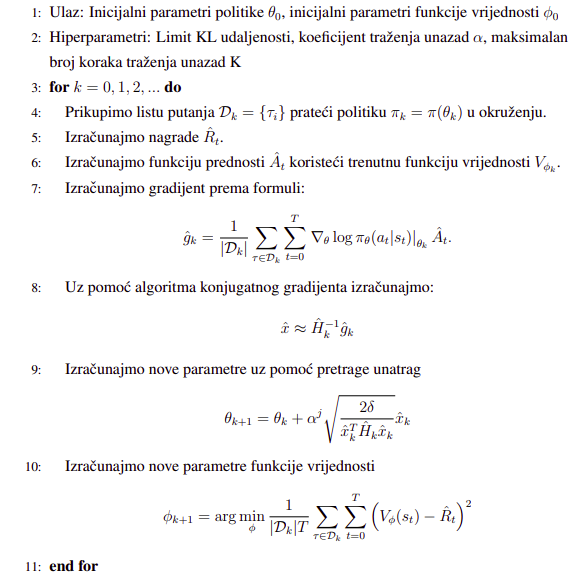
\includegraphics[height=8cm]{img/trpo.png}
	\end{figure}

\end{frame}


\subsection{Algoritam proksimalne optimizacije politike}

\begin{frame}
	\frametitle{Algoritam proksimalne optimizacije politike}

	\begin{figure}[h!]
		\centering
		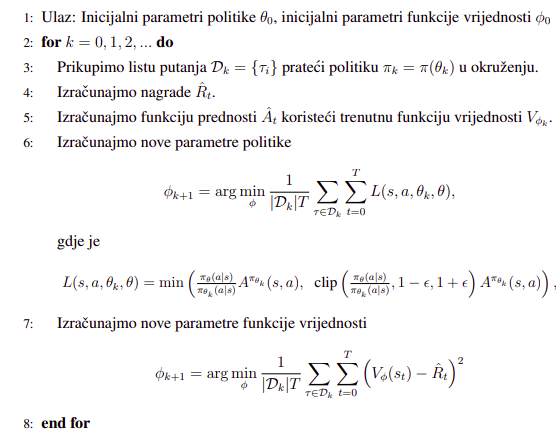
\includegraphics[width=\columnwidth]{img/ppo.png}
	\end{figure}

\end{frame}


\section{Inverzna kinematika robotske ruke Jaco}

\begin{frame}
	\frametitle{Robotski manipulatori}

	Robotski manipulatori sastoje se od čvrstih tijela koji su međusobno povezanih zglobovima.
	\bigskip

	Upravljanje robotima se dijeli na direktnu i inverznu kinematiku.
	\bigskip

	Jaco je učvršćen za podlogu, ima šest zglobova na čijem vrhu se nalazi efektor, a robotom se upravlja tako da se zadaju brzine zglobova.

\end{frame}

\begin{frame}
	\frametitle{Robotska ruka Jaco}

	\begin{figure}[ht!]
		\centering
		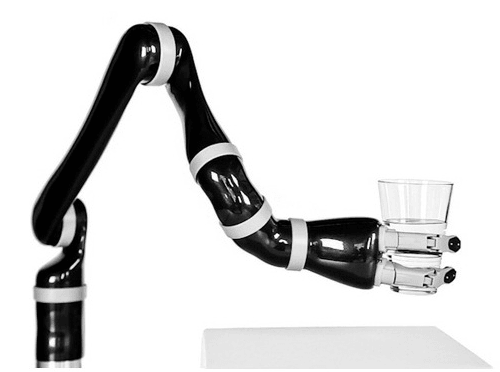
\includegraphics[width=0.9\columnwidth]{img/jaco.png}
		\label{fig:jaco}
	\end{figure}
	\footnotetext{Preuzeto sa \url{https://smashingrobotics.com}}

\end{frame}

\begin{frame}
	\frametitle{Problem dohvaćanja objekta}

	Cilj problema je efektorom robotske ruke doći do objekta, prvo u prostoru bez prepreka, onda s preprekama.
	\bigskip

	Prostor opservacija će se sastojati od položaja efektora, cilja i prepreka, a prostor akcija će biti šest brzina zglobova.

\end{frame}

\begin{frame}
	\frametitle{Implementacija manipulatora u simulatoru}

	Robotska ruka Jaco ostvarena je u simulatoru s programskim jezikom Python i njegovim bibliotekama.
	\bigskip

	Fizički model ostvaren je uz pomoć PyBulleta i Pyb-Manipulatora, a algoritmi su ostvareni uz pomoć Gyma i Baselinesa.
	\bigskip

	Ovo je sve trebalo povezati u okruženje za treniranje te pronaći odgovarajuću funkciju nagrade, odnosno gubitka.

\end{frame}

\begin{frame}
	\frametitle{Problem bez prepreka}

	\begin{figure}[ht!]
		\centering
		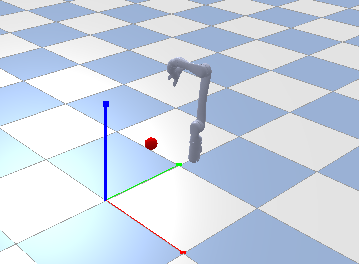
\includegraphics[width=\columnwidth]{img/bezprepreka.png}
		\label{fig:bezprepeka}
	\end{figure}

\end{frame}

\begin{frame}
	\frametitle{Problem s preprekama}

	\begin{figure}[ht!]
		\centering
		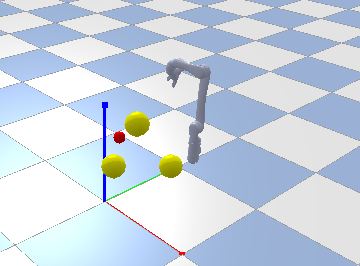
\includegraphics[width=\columnwidth]{img/spreprekama.png}
		\label{fig:sprepekama}
	\end{figure}

\end{frame}


\section{Rezultati}
\subsection{Izlaz agenta}

\begin{frame}
	\frametitle{Izlaz agenta}

	\begin{table}[ht!]
		\centering
		\label{tab:izlaz_agenta}
		\begin{tabular}{@{}ll@{}}
			\hline
			Ime parametra            & Vrijednost \\
			\hline
			\hline
			eplenmean                & 5e+03      \\
			eprewmean                & -5.09e+03  \\
			fps                      & 5.54e+03   \\
			loss/approxkl            & 0.0064     \\
			loss/clipfrac            & 0.0686     \\
			loss/policy\_entropy     & 8.43       \\
			loss/policy\_loss        & -0.0045    \\
			loss/value\_loss         & 104        \\
			misc/explained\_variance & 0.00614    \\
			misc/nupdates            & 3          \\
			misc/serial\_timesteps   & 6.14e+03   \\
			misc/time\_elapsed       & 141        \\
			misc/total\_timesteps    & 7.86e+05   \\
			\hline
		\end{tabular}
	\end{table}

\end{frame}

\subsection{Problem bez prepreka}

\begin{frame}[fragile]
	\frametitle{Udaljenost i brzina}

	\begin{figure}[h!]
		\centering
		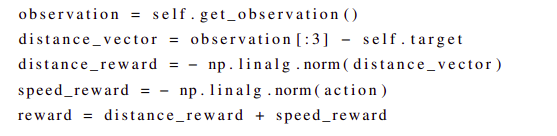
\includegraphics[width=\columnwidth]{img/ub.png}
	\end{figure}

\end{frame}

\begin{frame}
	\frametitle{Udaljenost i brzina}

	\begin{table}[ht!]
		\centering
		\label{tab:rub}
		\begin{tabular}{@{}lll@{}}
			\hline
			eplenmean & eprewmean & misc/total\_timesteps \\
			\hline
			\hline
			5001.00   & -4644.67  & 1.57e+06              \\
			5001.00   & -4405.25  & 2.88e+06              \\
			4934.95   & -4400.78  & 4.19e+06              \\
			5001.00   & -4487.64  & 5.51e+06              \\
			4976.26   & -4392.46  & 6.82e+06              \\
			4860.11   & -4157.88  & 8.13e+06              \\
			4916.93   & -4253.58  & 9.44e+06              \\
			4879.62   & -4589.74  & 1.07e+07              \\
			4953.33   & -4476.76  & 1.21e+07              \\
			4911.33   & -4511.79  & 1.34e+07              \\
			4862.73   & -4430.52  & 1.47e+07              \\
			4928.81   & -4643.92  & 1.60e+07              \\
			4973.91   & -4636.84  & 1.73e+07              \\
			5001.00   & -4764.21  & 1.86e+07              \\
			4968.79   & -4585.88  & 1.99e+07              \\
			\hline
		\end{tabular}
	\end{table}

\end{frame}

\begin{frame}
	\frametitle{Napredak i brzina}

	\begin{figure}[h!]
		\centering
		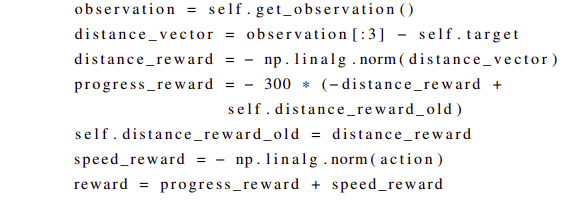
\includegraphics[width=\columnwidth]{img/nb.png}
	\end{figure}

\end{frame}

\begin{frame}
	\frametitle{Napredak i brzina}

	\begin{table}[ht!]
		\centering
		\label{tab:rub}
		\begin{tabular}{@{}lll@{}}
			\hline
			eplenmean & eprewmean & misc/total\_timesteps \\
			\hline
			\hline
			4558.74   & -2145.22  & 1.57e+06              \\
			3990.53   & -1814.93  & 2.88e+06              \\
			1933.10   & -884.44   & 4.19e+06              \\
			1260.32   & -582.99   & 5.51e+06              \\
			1300.25   & -597.80   & 6.82e+06              \\
			1016.17   & -468.28   & 8.13e+06              \\
			885.16    & -409.56   & 9.44e+06              \\
			824.18    & -381.70   & 1.07e+07              \\
			928.05    & -428.19   & 1.21e+07              \\
			890.89    & -412.20   & 1.34e+07              \\
			793.56    & -358.08   & 1.47e+07              \\
			854.25    & -394.39   & 1.60e+07              \\
			711.99    & -326.41   & 1.73e+07              \\
			746.49    & -337.91   & 1.86e+07              \\
			791.45    & -361.71   & 1.99e+07              \\
			\hline
		\end{tabular}
	\end{table}

\end{frame}

\begin{frame}
	\frametitle{Udaljenost, napredak i brzina}

	\begin{figure}[h!]
		\centering
		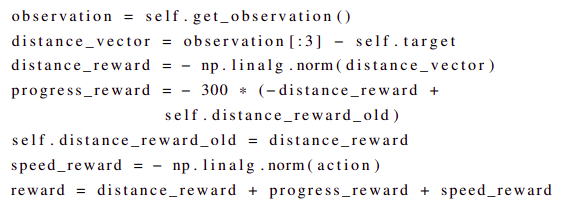
\includegraphics[width=\columnwidth]{img/unb.png}
	\end{figure}

\end{frame}

\begin{frame}
	\frametitle{Udaljenost, napredak i brzina}

	\begin{table}[ht!]
		\centering
		\label{tab:rub}
		\begin{tabular}{@{}lll@{}}
			\hline
			eplenmean & eprewmean & misc/total\_timesteps \\
			\hline
			\hline
			3819.96   & -3031.81  & 1.57e+06              \\
			3578.17   & -2906.71  & 2.88e+06              \\
			2264.80   & -1710.63  & 4.19e+06              \\
			1791.30   & -1360.40  & 5.51e+06              \\
			1497.91   & -1119.63  & 6.82e+06              \\
			1110.11   & -774.56   & 8.13e+06              \\
			971.30    & -714.09   & 9.44e+06              \\
			977.26    & -753.41   & 1.07e+07              \\
			1102.77   & -832.46   & 1.21e+07              \\
			830.59    & -669.11   & 1.34e+07              \\
			779.17    & -604.76   & 1.47e+07              \\
			773.30    & -599.63   & 1.60e+07              \\
			807.47    & -645.58   & 1.73e+07              \\
			719.24    & -580.12   & 1.86e+07              \\
			701.33    & -577.36   & 1.99e+07              \\
			\hline
		\end{tabular}
	\end{table}

\end{frame}

\subsection{Problem s preprekama}

\begin{frame}
	\frametitle{Linearno kažnjavanje blizine i fiksne nagrade na kraju epizode}

	\begin{figure}[h!]
		\centering
		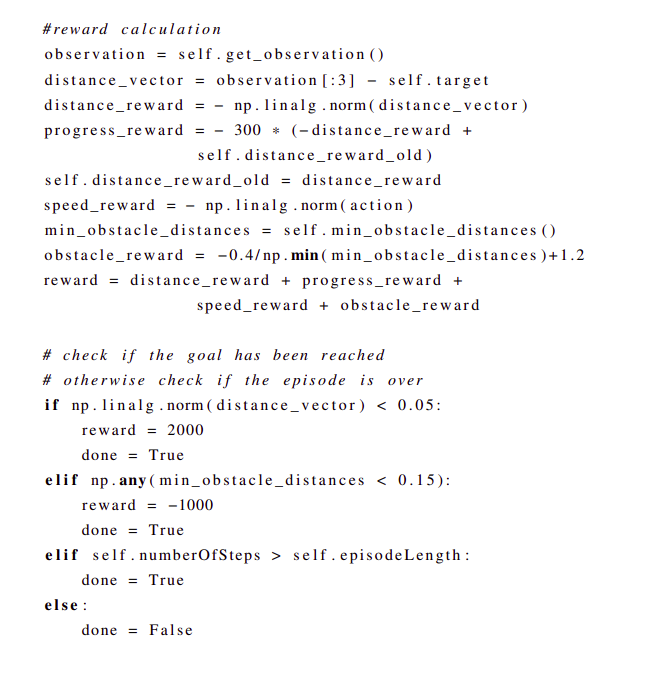
\includegraphics[height=8cm]{img/fix.png}
	\end{figure}

\end{frame}

\begin{frame}
	\frametitle{Linearno kažnjavanje blizine i fiksne nagrade na kraju epizode}

	\begin{table}[ht!]
		\centering
		\label{tab:rub}
		\begin{tabular}{@{}lll@{}}
			\hline
			eplenmean & eprewmean & misc/total\_timesteps \\
			\hline
			\hline
			4660.64   & -4230.35  & 1.57e+06              \\
			4067.72   & -3506.76  & 2.88e+06              \\
			3041.90   & -2856.47  & 4.19e+06              \\
			3681.57   & -3091.60  & 5.51e+06              \\
			3496.40   & -3116.02  & 6.82e+06              \\
			3568.77   & -3106.93  & 8.13e+06              \\
			3296.14   & -2790.05  & 9.44e+06              \\
			3704.81   & -2935.27  & 1.07e+07              \\
			3625.26   & -3061.75  & 1.21e+07              \\
			3196.91   & -2385.26  & 1.34e+07              \\
			2445.88   & -1936.88  & 1.47e+07              \\
			2597.89   & -1847.29  & 1.60e+07              \\
			2053.09   & -1335.68  & 1.73e+07              \\
			1389.56   & -628.74   & 1.86e+07              \\
			1786.80   & -1134.73  & 1.99e+07              \\
			\hline
		\end{tabular}
	\end{table}

\end{frame}

\begin{frame}
	\frametitle{Linearno kažnjavanje blizine i bez završavanja prilikom udarca u prepreku}

	\begin{figure}[h!]
		\centering
		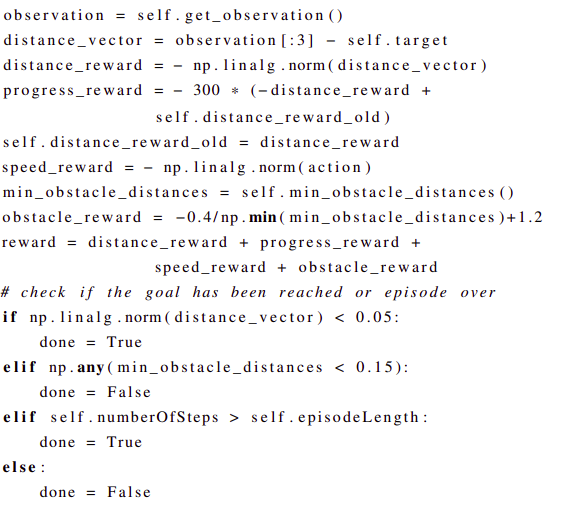
\includegraphics[height=8cm]{img/bes.png}
	\end{figure}

\end{frame}

\begin{frame}
	\frametitle{Linearno kažnjavanje blizine i bez završavanja prilikom udarca u prepreku}

	\begin{table}[ht!]
		\centering
		\label{tab:rub}
		\begin{tabular}{@{}lll@{}}
			\hline
			eplenmean & eprewmean & misc/total\_timesteps \\
			\hline
			\hline
			4853.53   & -9865.14  & 1.57e+06              \\
			4960.64   & -10915.79 & 2.88e+06              \\
			4919.95   & -9538.70  & 4.19e+06              \\
			4625.72   & -8614.35  & 5.51e+06              \\
			4683.32   & -9372.60  & 6.82e+06              \\
			4557.16   & -8919.95  & 8.13e+06              \\
			4165.51   & -7997.34  & 9.44e+06              \\
			4299.81   & -8486.60  & 1.07e+07              \\
			4245.40   & -8459.33  & 1.21e+07              \\
			3756.71   & -7258.29  & 1.34e+07              \\
			4494.71   & -8596.00  & 1.47e+07              \\
			4400.12   & -7979.35  & 1.60e+07              \\
			4069.01   & -7443.17  & 1.73e+07              \\
			4042.78   & -7213.07  & 1.86e+07              \\
			3930.52   & -7177.77  & 1.99e+07              \\
			\hline
		\end{tabular}
	\end{table}

\end{frame}

\begin{frame}
	\frametitle{Eksponencijalno kažnjavanje blizine i bez završavanja prilikom udarca u prepreku}

	\begin{figure}[h!]
		\centering
		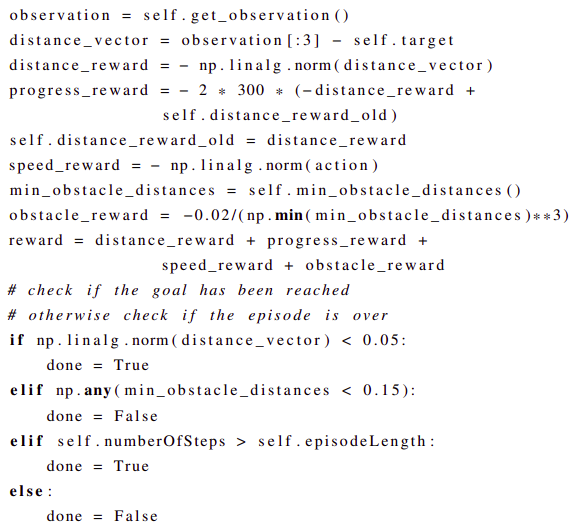
\includegraphics[height=8cm]{img/eksp.png}
	\end{figure}

\end{frame}

\begin{frame}
	\frametitle{Eksponencijalno kažnjavanje blizine i bez završavanja prilikom udarca u prepreku}

	\begin{table}[ht!]
		\centering
		\label{tab:rub}
		\begin{tabular}{@{}lll@{}}
			\hline
			eplenmean & eprewmean & misc/total\_timesteps \\
			\hline
			\hline
			4877.34   & -11253.18 & 1.57e+06              \\
			4679.16   & -10129.53 & 2.88e+06              \\
			4122.46   & -9429.34  & 4.19e+06              \\
			3730.75   & -8085.56  & 5.51e+06              \\
			4014.43   & -7986.74  & 6.82e+06              \\
			3106.13   & -6309.29  & 8.13e+06              \\
			3120.73   & -6476.75  & 9.44e+06              \\
			1998.13   & -3773.81  & 1.07e+07              \\
			1702.80   & -2987.62  & 1.21e+07              \\
			2300.74   & -4048.41  & 1.34e+07              \\
			2318.29   & -4525.41  & 1.47e+07              \\
			1770.62   & -3393.89  & 1.60e+07              \\
			2229.36   & -4106.26  & 1.73e+07              \\
			1683.42   & -3848.00  & 1.86e+07              \\
			1239.36   & -2636.43  & 1.99e+07              \\
			\hline
		\end{tabular}
	\end{table}

\end{frame}

\begin{frame}
	\frametitle{Eksponencijalno kažnjavanje blizine i bez završavanja prilikom udarca u prepreku}

	\begin{table}[ht!]
		\centering
		\label{tab:rub}
		\begin{tabular}{@{}lll@{}}
			\hline
			eplenmean & eprewmean & misc/total\_timesteps \\
			\hline
			\hline
			4661.85   & -9838.50  & 2.88e+06              \\
			4137.11   & -8440.07  & 5.51e+06              \\
			3791.15   & -7692.32  & 8.13e+06              \\
			2962.36   & -5753.18  & 1.07e+07              \\
			2715.98   & -5039.09  & 1.34e+07              \\
			2221.33   & -4388.06  & 1.60e+07              \\
			1667.47   & -3272.12  & 1.86e+07              \\
			1704.15   & -3254.69  & 2.12e+07              \\
			1323.04   & -2676.78  & 2.39e+07              \\
			1401.51   & -2744.61  & 2.65e+07              \\
			1364.24   & -2430.31  & 2.91e+07              \\
			1106.77   & -2208.91  & 3.17e+07              \\
			1154.20   & -2399.01  & 3.43e+07              \\
			1256.99   & -2446.23  & 3.70e+07              \\
			1100.65   & -2358.74  & 3.96e+07              \\
			\hline
		\end{tabular}
	\end{table}

\end{frame}

\begin{frame}
	\frametitle{Eksponencijalno kažnjavanje blizine i bez završavanja prilikom udarca u prepreku}

	\begin{table}[ht!]
		\centering
		\label{tab:rub}
		\begin{tabular}{@{}lll@{}}
			\hline
			eplenmean & eprewmean & misc/total\_timesteps \\
			\hline
			\hline
			4887.21   & -16079.80 & 2.88e+06              \\
			4490.02   & -12362.30 & 5.51e+06              \\
			4715.55   & -17295.69 & 8.13e+06              \\
			4389.97   & -14387.87 & 1.07e+07              \\
			3545.18   & -10016.69 & 1.34e+07              \\
			3276.90   & -10959.46 & 1.60e+07              \\
			2771.84   & -7745.69  & 1.86e+07              \\
			2524.67   & -8585.83  & 2.12e+07              \\
			2393.39   & -7386.62  & 2.39e+07              \\
			2620.81   & -8626.77  & 2.65e+07              \\
			2077.17   & -6748.79  & 2.91e+07              \\
			2084.14   & -7185.85  & 3.17e+07              \\
			1545.79   & -5538.39  & 3.43e+07              \\
			1880.94   & -6492.34  & 3.70e+07              \\
			1663.24   & -5263.44  & 3.96e+07              \\
			\hline
		\end{tabular}
	\end{table}

\end{frame}

\section{Zaključak}
\begin{frame}
	\frametitle{Zaključak}

	Problem inverzne kinematike riješili smo pomoću dubokog potpornog učenja, no povećanjem težine zadataka, rješavanje problema postaje još teže.
	\bigskip
	
	Prije desetak godina, kada je umjetna inteligencija uzela maha, jako mnogo se pričalo o takozvanoj "tehnološkoj singularnosti", točki u vremenu kada će računala poprimiti vlastitu svijest i postati ravnopravna ljudima.
	\bigskip

	Mišljenja sam da ako će nas išta dovesti do "tehnološke singularnosti", onda je to duboko potporno učenje.

\end{frame}



\begin{frame}
	\begin{center}
		\Huge Hvala na pažnji!
	\end{center}
\end{frame}

\end{document}
